% !TEX encoding = UTF-8
% !TEX TS-program = pdflatex
% !TEX root = ../tesi.tex

%**************************************************************
\chapter{L'applicazione}
\label{cap:applicazione}
%**************************************************************

%\intro{Breve introduzione al capitolo}\\

\section{Introduzione alle grammatiche}
Zucchetti negli ultimi anni ha investito molto nella ricerca di una tecnologia che gli permettesse di interagire con i propri prodotti attraverso comandi vocali ed ora sta realizzando delle regole che consentono di generare un numero di \emph{grammatiche} potenzialmente infinito e capace di comprendere ed elaborare il linguaggio naturale.
Gli assistenti virtuali presenti sul mercato sono basati sul seguente concetto: provare a capire tutto ciò che viene detto dagli utenti anche a costo di commettere degli errori. Questa filosofia è mirata a dare all'utente la sensazione di utilizzare uno strumento in grado di capire e ragionare in qualsiasi momento ed è già utilizzata in larga scala da grandi aziende quali Google, Amazon e Apple. Tuttavia, per le funzionalità della maggior parte dei prodotti Zucchetti, tale principio non è applicabile. Infatti necessitano che, quando una frase viene riconosciuta e compresa, il margine di errore sia nullo. Un classico esempio è il trasferimento di denaro in cui se la comprensione del comando avviene in modo errato c'è il rischio di causa danni contingenti agli utenti. \\
Dunque Zucchetti ha intrapreso una strada diversa sviluppando una tecnologia mirata a alla massima precisione accettando talvolta di non riconoscere i comandi ricevuti. Essa consiste quindi in regole molto semplici ed intuitive da applicare a stringhe di testo e riassunte in quattro azioni principali:
\begin{itemize}
	\item concatenazione di elementi;
	\item scelta tra più elementi;
	\item ripetizione di uno o più elementi;
	\item opzionalità di un elemento.
\end{itemize}
A partire da ciò viene costruita una \emph{\gls{gramg}} che permette di interpretare un insieme finito di frasi che rappresentano il dominio della conversazione che si vuole intrattenere. La difficoltà principale è comprendere esattamente l'insieme delle possibili frasi, trovate con un'analisi probabilistica e statistica sul proprio contesto, che si presume l'utente possa dire, senza includere componenti non pertinenti. \\
Un esempio semplice ma dimostrativo di una \emph{\gls{gramg}} che permette di interpretare alcune frasi di saluto è illustrato nella seguente immagine.

\begin{figure}[htbp]
	\begin{center}
		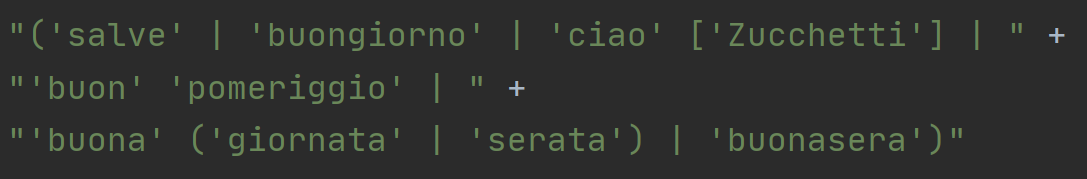
\includegraphics[height=2cm, width=\linewidth]{esempio-grammatica.PNG}
		\caption{Esempio di una grammatica}
	\end{center}
\end{figure}

\vspace{2cm}

Nonostante il loro principio di funzionamento sia relativamente semplice da comprendere, non sono altrettanto facili da interpretare qualora raggiungessero grandi dimensioni e, a maggior ragione, per uno sviluppatore terzo che in futuro le dovrà riutilizzare. Per migliorare questo aspetto l'azienda ha quindi deciso di utilizzare i diagrammi \emph{\gls{rldg}}\glsfirstoccur come strumento di rappresentazione come si può vedere nella figura successiva.

\begin{figure}[htbp]
	\begin{center}
		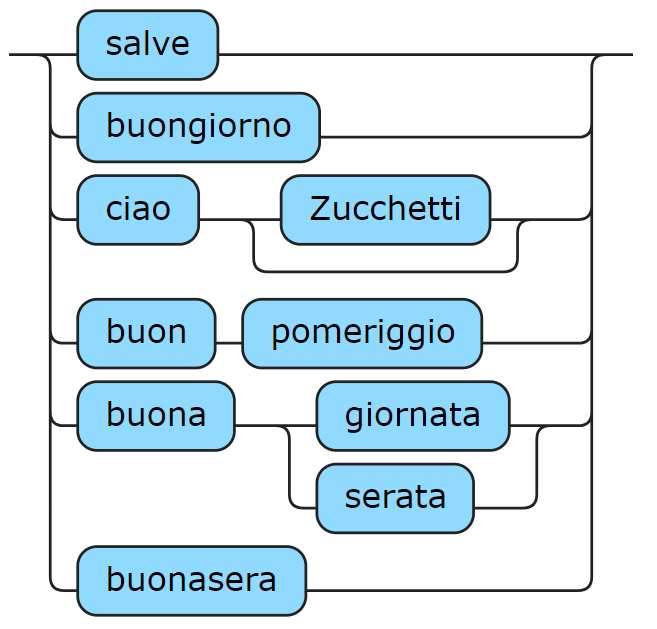
\includegraphics[height=6cm]{esempio-railroad.PNG}
		\caption{Esempio di una grammatica con railroad}
	\end{center}
\end{figure}

Risulta evidente come questa raffigurazione sia molto più efficace e intuitiva. \\
Infine l'applicazione della \emph{\gls{gramg}} sui comandi vocali dell'utente tradotti in stringa avviene attraverso un apposito \emph{\gls{parsg}}\glsfirstoccur sviluppato da Zucchetti che mi è stato consegnato per lo sviluppo del mio progetto.
\section{Analisi dei requisiti}
	\subsection{Descrizione del problema}
	Durante l'attività di ricerca ed analisi sugli assistenti virtuali, in particolare nello sviluppo del \emph{\gls{pocg}} che fa uso di Alexa, è emerso un concetto caratteristico anche del lavoro che sta svolgendo l'azienda: la conversazionalità. Essa rappresenta la capacità di intrattenere una conversazione da parte di un software simulando la presenza di una persona. \\
	Successivamente è stato pianificato di costruire una propria \emph{\gls{nlug}} con una \emph{\gls{gramg}} che interpreti un insieme di frasi e dia una risposta ragionata sulla base di esse. \\
	È stato quindi deciso in accordo con il tutor di costruire un'applicazione che metta assieme la realizzazione di una propria \emph{\gls{nlug}} con capacità di conversazione finalizzata al soddisfacimento di una determinata funzionalità e non limitata ad una coppia domanda-risposta. Il dominio è simile a quello del \emph{\gls{pocg}} sviluppato con Alexa ovvero la data di nascita solo che molto più completo. Le frasi pronunciabili dagli utenti di cui è prevista la comprensione sono  composte da:
	\begin{itemize}
		\item saluto iniziale opzionale;
		\item un insieme completo di frasi introduttive per esprimere la data di nascita nel formato giorno, mese e anno o, alternativamente, la data di compleanno nel formato giorno, mese;
		\item insieme completo di espressioni per la data di nascita e conseguentemente del sottoinsieme data di compleanno;
		\item insieme di frasi per riconoscere come data il giorno di Natale;
		\item insieme di frasi per riconoscere come data il primo giorno di un qualsiasi mese;
		\item insieme di frasi per interrompere in qualunque momento l'esecuzione;
		\item insieme di frasi per chiedere un eventuale aiuto sulle funzionalità dell'applicazione.
	\end{itemize}
	\subsection{Requisiti}
	Lo scopo principale è dimostrare la fattibilità di implementare la capacità conversazionale in una \emph{\gls{nlug}} costruita con la tecnologia sviluppata da Zucchetti. L'applicazione perciò si presenta sotto forma di \emph{\gls{pocg}} e non è quindi integrata in un software aziendale esistente. \\
	Analizzando più in dettaglio gli obiettivi da raggiungere, è stata stilata una lista di requisiti obbligatori la cui fattibilità è certa. Uno stra quelli emersi, invece, è stato inserito come opzionale poiché rappresenta un miglioramento ragionevolmente non implementabile nel tempo a disposizione.
	I requisiti obbligatori sono i seguenti:
	\begin{enumerate}
		\item costruzione dell'interfaccia utente:
			\begin{itemize}
				\item interfaccia grafica minimale che permetta all'utente di attivare il riconoscimento del comando vocale;
				\item interfaccia vocale completa di tutti gli accessori studiati durante l'attività di ricerca. Risulta essere in input una diretta conseguenza dello sviluppo della \emph{\gls{nlug}} mentre in output deve essere progettata dallo sviluppatore sulla base delle elaborazioni prodotte.
			\end{itemize}
		\item costruzione di una \emph{\gls{nlug}} che comprenda la data di nascita espressa dall'utente, esegua un'elaborazione e prepari una risposta adatta. Deve avere estrema precisione del comprendere le frasi una volta riconosciute anche a costo di rigettarne alcune;
		\item implementazione della capacità conversazionale con memoria al fine di portare a compimento la funzionalità in esecuzione dando maggiormente la percezione all'utente di dialogare con una persona. %TODO: SPIEGARE CHE DEVO OTTENERE LA DATA INTERA E QUINDI RICHIEDO
	\end{enumerate}
	Il requisito opzionale è il seguente:
	\begin{itemize}
		\item generalizzazione della grammatica in modo che permetta non solo di interpretare l'input dell'utente ma anche di generare la risposta sulla base dell'elaborazione.
	\end{itemize}
\section{Progettazione}
	\subsection{NLU}
	La \emph{\gls{nlug}} è il nucleo di tutto l'applicativo e la sua corretta progettazione è fondamentale. Essa consiste nella generazione della \emph{\gls{gramg}} che interpreta l'input dell'utente ed è rappresentata nel seguente diagramma \emph{\gls{rldg}}.
	
	%TODO: SCHEMA INTERFACCIA VOCALE
	
	%TODO: DESCRIZIONE DEL DIAGRAMMA RAILROAD
	\subsection{Capacità conversazionale}
	Per l'implementazione della capacità conversazionale il concetto fondamentale è la memoria. Mentre la \emph{\gls{nlug}} permette l'interpretazione del linguaggio naturale, la capacità conversazionale consiste nel mantenere il contesto durante l'intero dialogo. Ho deciso di tenerne traccia all'interno di un oggetto da resettare ad ogni nuova conversazione, in questo modo nella costruzione delle risposte è possibile far uso di tali dati per porre domande mirate al fine di ottenere i dati mancanti che in questo caso specifico possono essere giorno, mese e anno.
	\subsection{Interfaccia utente}
	La progettazione dell'interfaccia utente si articola in due parti:
	\begin{itemize}
		\item interfaccia grafica;
		\item interfaccia vocale.
	\end{itemize}
		\subsubsection{Interfaccia grafica}
		L'interfaccia grafica è stata progettata con un numero di elementi minimali all'interno ed è illustrata nella seguente immagine.
		
		\begin{figure}[htbp]
			\begin{center}
				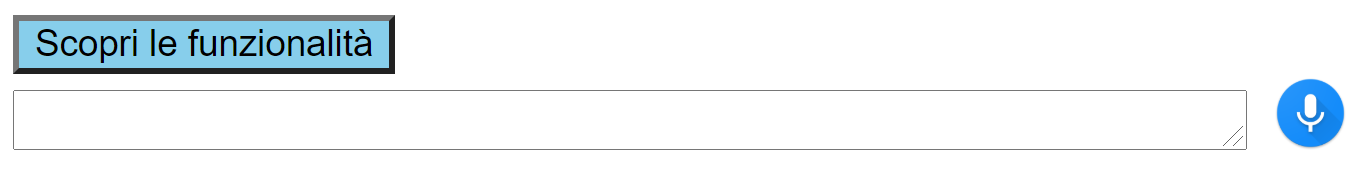
\includegraphics[height=2cm, width=\linewidth]{interfaccia-grafica.PNG}
				\caption{Interfaccia grafica dell'applicazione}
			\end{center}
		\end{figure}
	
		I componenti infatti sono un pulsante che permette all'utente di ascoltare le funzionalità fornite, un pulsante con l'immagine del microfono che attiva il riconoscimento vocale ed infine una casella di testo non editabile che permetta di visualizzare il comando che è stato riconosciuto.		
		\subsubsection{Interfaccia vocale}
		L'interfaccia vocale è stata progettata con l'obiettivo di garantire un'esperienza d'uso migliore possibile agli utenti. Ho utilizzato le nozioni apprese dalla documentazione degli assistenti virtuali analizzati per generare un'interfaccia vocale e sono:
		\begin{itemize}
			\item %TODO: CERCA COME FARE INTEFACCIA VOCALE DA GOOGLE/ALEXA
		\end{itemize}		
		Tutti i componenti espressi nell'analisi sono quindi stati progettati. In particolare i comandi corrispondenti all'interruzione forzata dell'applicazione e alla richiesta d'aiuto che sono stati utilizzati risultano un'elaborazione di un sottoinsieme di quelli ricavati da un'analisi comportamentale di Zucchetti sugli utenti, qualora siano tranquilli e rilassati ma anche arrabbiati e agitati. \\
		Per gli input dell'utente l'interfaccia vocale è realizzata automaticamente a partire dalla progettazione della \emph{\gls{gramg}} per la quale sono comunque stati applicati i principi descritti mentre per l'output è stata personalizzata sulla base dell'elaborazione. Si è quindi deciso di fornire un set di frasi con significato uguale ma con una sintassi leggermente diversa da cui viene scelta al momento la frasi di input secondo un algoritmo pseudo-casuale.
\section{Codifica}

\section{Test}

\section{Sviluppi futuri}
Sarebbe stato possibile tenere traccia dei dati forniti dall'utente in modo permanente ad esempio all'interno di un database così che ad un nuovo utilizzo dell'utente l'applicazione si ricordasse di ciò che era stato detto precedentemente. Questo però pone alcuni vincoli quali un sistema di autenticazione dell'utente perciò diventa complesso.